\documentclass[xcolor=dvipsnames, handout]{beamer}

\usepackage[utf8x]{inputenc}
\usepackage{default}
\usetheme[width=50pt]{ULatina}   % Bergen, Darmstadt
\usecolortheme[named=Green]{structure}
\usepackage{graphicx}
\usepackage{pgfpages}
\usepackage{tikz}
\usepackage[spanish]{babel}

\newcommand{\uC}{\ensuremath{\mu\textrm{C}}\ }
\newcommand{\iic}{I\ensuremath{^2}C\ }
\newcommand{\pageframe}[1]{\frame{\begin{center}{ \Huge #1 }\end{center}}}
\newcommand{\rtl}{\ensuremath{\leftarrow}}
\newcommand{\ltr}{\ensuremath{\rightarrow}}
\newcommand{\bidir}{\ensuremath{\leftrightarrow}}

%\setbeameroption{show notes on second screen}

\title[Buses]{Buses y protocolos de comunicación}
%\subtitle[]{}
\author{Prof. Jorge Rivera~Guti\'errez}
\institute{Universidad Latina de Costa Rica\\ Ingenier\'\i a en Electr\'onica}
\logo{\includegraphics[height=45pt]{world.png}}
\date{II Cuatrimestre 2015}

\PrerenderUnicode{ó}
\def\svgwidth{\textwidth}

\begin{document}

\begin{frame}
 \maketitle
\end{frame}

\begin{frame}
 \tableofcontents
\end{frame}

\section{Buses paralelos}

\pageframe{Buses paralelos}

\pageframe{LPT, IEEE-1284, etc.}

\begin{frame}{IEEE-1284}
  \begin{block}{Puerto paralelo (LPT)}
    \begin{itemize}[<+->]
      \item Originalmente para impresoras, unidireccional
      \item Usualmente utiliza un conector DB-25
      \item Muy específico
    \end{itemize}
  \end{block}
  \only<2>{
  \begin{center}
    \includegraphics[width=0.6\textwidth]{parallel-db25}
  \end{center}}
\end{frame}

\begin{frame}{IEEE-1284}
  \begin{block}{Señales}
    \begin{center}
    \begin{tabular}{|c|p{0.5\textwidth}|c|}\hline
      Pin	& Nombre	& Dir	\\\hline\hline
      1		& /Strobe	& \bidir \\\hline
      2-9	& Data0-Data7	& \ltr	\\\hline
      10	& Ack		& \rtl	\\\hline
      11	& /Busy		& \rtl	\\\hline
      12	& Paper-Out	& \rtl	\\\hline
      13	& Select	& \rtl	\\\hline
      14	& /Linefeed	& \bidir \\\hline
      15	& Error		& \rtl 	\\\hline
      16	& Reset		& \bidir \\\hline
      17	& /Select-Printer& \bidir \\\hline
      18-25	& Ground	& \\\hline

    \end{tabular}
    \end{center}
  \end{block}
\end{frame}

\pageframe{Memorias}

\begin{frame}{Memoria}
  \begin{block}{RAM/ROM/Flash\ldots}
    \begin{itemize}[<+->]
      \item Buses de datos/direcciones (separados o multiplexados)
      \item Señales de control (RD/WR/CS/ALE)
      \item 1 ``Master''
      \item 1+ ``Slave''
      \item Tamaño de memoria limitado por bus de direcciones
      \item Requiere de muchas líneas
      \item Útil para tarjetas, pero no para conexión externa
    \end{itemize}
  \end{block}
\end{frame}


\pageframe{PSP}

\begin{frame}{PSP}
  \begin{block}{Parallel Slave Port}
    \begin{itemize}[<+->]
      \item Permite a un PIC actuar como memoria externa
      \item Solo funciona en modo esclavo
      \item Conexión de múltiples dispositivos en un sistema
    \end{itemize}
  \end{block}  
\end{frame}

\begin{frame}{PSP}
  \begin{block}{Operación write}
    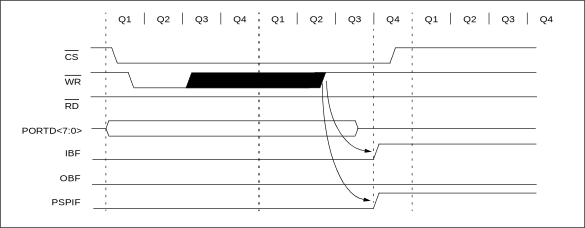
\includegraphics[width=\textwidth]{psp-write}
  \end{block}
\end{frame}

\begin{frame}{PSP}
  \begin{block}{Operación read}
    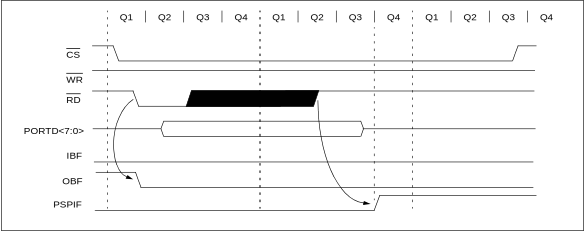
\includegraphics[width=\textwidth]{psp-read.pdf}
  \end{block}
\end{frame}

\begin{frame}{PSP}
  \begin{block}{Registros}
    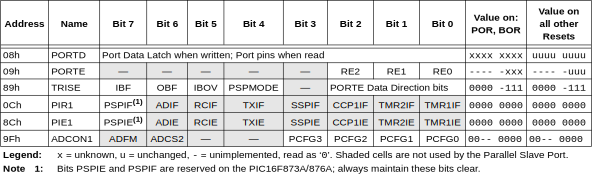
\includegraphics[width=\textwidth]{psp-regs}
  \end{block}
\end{frame}


\section{Buses serie}

\pageframe{Buses serie}

\pageframe{RS-232}

\begin{frame}{TIA-232}
  \begin{block}{\textit{RS}-232}
    \begin{itemize}[<+->]
      \item Estándar recomendado 232
      \item Usualmente usa conector DB-9
      \item DCE: Data Circuit-Terminating Equipment (Módem)
      \item DTE: Data Terminal Equipment (PC)
      \item Niveles de tensión: $\pm$3V hasta $\pm$25V
      \item Comunicación asincrónica
      \item 9600, 19200, 38400, 115200 bauds
    \end{itemize}
  \end{block}

  \only<2>{
  \begin{center}
    \includegraphics[width=0.3\textwidth]{serial-db9}
  \end{center}}

\end{frame}

\begin{frame}{TIA-232}
  \begin{block}{Modos de funcionamiento}
    \begin{itemize}[<+->]
      \item ``Endianness'' (\textbf{Little-Endian}, Big-Endian)
      \item Número de bits (5,6,7,\textbf{8},9)
      \item Paridad (\textbf{None}, Odd, Even, Mark, Space)
      \item Bits de parada (\textbf{1}, 1.5, 2)
      \item Control de Flujo
    \end{itemize}
  \end{block}

  \only<6->{
  \begin{block}{Notación convencional}
    \begin{itemize}[<+->]
      \item 8/N/1
      \item 7/E/1
      \item 9/O/2
    \end{itemize}

  \end{block}}

\end{frame}


\begin{frame}{TIA-232}
  \begin{block}{Señales}
    \begin{tabular}{|l|c|c|}\hline
      Nombre			& Dirección	& Pin (DB9) \\\hline\hline
      Data Terminal Ready (DTR) & DTE \ltr DCE	& 4 \\\hline
      Data Carrier Detect (DCD)	& DTE \rtl DCE 	& 1 \\\hline
      Data Set Ready (DSR)	& DTE \rtl DCE 	& 6 \\\hline
      Ring Indicator (RI)	& DTE \rtl DCE 	& 9 \\\hline
      Request to Send (RTS)	& DTE \ltr DCE 	& 7 \\\hline
      Clear to Send (CTS)	& DTE \rtl DCE 	& 8 \\\hline
      \textbf{Transmitted Data (TxD)}	& DTE \ltr DCE 	& 2 \\\hline
      \textbf{Received Data (RxD)}	& DTE \rtl DCE 	& 3 \\\hline
      \textbf{Ground (GND)}		& 		& 5 \\\hline	
    \end{tabular}
  \end{block}
\end{frame}


\begin{frame}{TIA-232}  
  \begin{block}{Forma de onda}
    \includegraphics[width=\textwidth]{rs232-trace}
  \end{block}
\end{frame}

\pageframe{\iic}

\begin{frame}{\iic}
  \begin{block}{\iic: Inter-Integrated Circuit}
    \begin{itemize}[<+->]
      \item También conocido como Two-Wire Interface (TWI)
      \item Utiliza solo dos cables
      \item Comunicación sincrónica
      \item Half-duplex
      \item 1+ maestros, 1+ esclavos
      \item Direcciones de 7 bits
      \item Hasta 128 direcciones, 112 dispositivos
      \item ``Big-endian''
      \item 100kb/s, 400kb/s, 1Mb/s
    \end{itemize}
  \end{block}
\end{frame}

\begin{frame}{\iic}
 \begin{block}{\iic}
  \begin{center}
   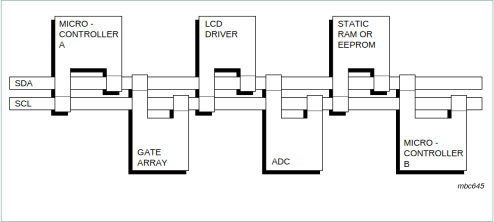
\includegraphics[width=\textwidth]{i2c-diag}
  \end{center}
 \end{block}
\end{frame}

\begin{frame}{\iic}
 \begin{block}{Conexión y funcionamiento}
  \begin{itemize}[<+->]
    \item Dos líneas: SDA y SCL
    \item Puertos open-drain
    \item Requiere resistencias de pull-up en las líneas
    \item Master controla el SCL
    \item Se utilizan señales de ACK para confirmar los datos
  \end{itemize}
 \end{block}

\end{frame}

\begin{frame}{\iic}
 \begin{block}{Formato de transmisión}
  \includegraphics[width=\textwidth]{i2c-trans}
 \end{block}

\end{frame}

\begin{frame}{\iic - Ejemplo}
\texttt{
\noindent\#include $<$Wire.h$>$\\
~\\
void setup() \{\\
~~Wire.begin();\\
~~Wire.beginTransmission(address);\\
~~Wire.send(0x0E);\\
~~Wire.send(0x00);\\
~~Wire.send(0x00);\\
~~Wire.send(0x80);\\
~~Wire.send(0xAA);\\
~~Wire.send(0xAA);\\
~~Wire.send(0x02);\\
~~resp = Wire.endTransmission();\\
\}
}
\end{frame}




\pageframe{SPI}

\begin{frame}{SPI}
  \begin{block}{SPI: Serial Peripheral Interface}
    \begin{itemize}[<+->]
     \item También conocido como 3-Wire o 4-Wire
      \item Utiliza 4 líneas de comunicación
      \item Full-duplex
      \item Un maestro, varios esclavos
      \item Requiere una línea SS por cada esclavo
      \item 1-70MHz
    \end{itemize}

  \end{block}
\end{frame}

\begin{frame}{SPI}
 \begin{block}{SPI}
  \begin{center}
\begin{tabular}{|c|p{0.6\textwidth}|}\hline
    Nombre	&	Descripción \\ \hline\hline
    SCLK	&	Serial Clock \\ \hline
    MOSI/SIMO	&	Master Out/Slave In\\ \hline
    MISO/SOMI	&	Master In/Slave Out\\ \hline
    SS		&	Slave Select\\ \hline
  \end{tabular}               \end{center}

 \end{block}

\end{frame}



\end{document}
